%28/10 - Fátima Sánchez Cabo
\chapter{Introducción a la genómica: caracterización del genoma mediante NGS}
\section{Introducción a la genómica traslacional}
\subsection{Definición e importancia de la genómica}
La genómica, el estudio integral del ADN y de la estructura, función y dinámica de los genomas, representa un pilar fundamental en la biología moderna. Marcó un cambio de paradigma, pasando de un enfoque reduccionista en biología - donde se estudiaban componentes individuales y de manera aislada - a una perspectiva integradora que analiza las interacciones y relaciones entre los distintos elementos biológicos. Esta transición permitió evolucionar de la genética clásica, basada en hipótesis concretas, hacia la genómica, que integra análisis de datos masivos sin necesidad de preguntas iniciales específicas, aunque sí en constante búsqueda de respuestas biológicas complejas.

En el marco del dogma central de la biología, las “ómicas” representan tres niveles de estudio: la genómica (centrada en el ADN), la transcriptómica (ARN) y la proteómica (proteínas). Este curso se enfoca en la genómica, ya que la información genética determina las funciones bioquímicas y, por ende, los fenotipos de los organismos. Gracias a avances recientes, ahora es posible inferir la función bioquímica de las proteínas directamente a partir de la secuencia de ADN, sin necesidad de técnicas complejas como la cristalización. Además, herramientas de inteligencia artificial pueden predecir la estructura de las proteínas con precisión, acelerando la interpretación de funciones biológicas.

Las proteínas, incluyendo enzimas esenciales, son los elementos funcionales clave en la biología. La secuencia de aminoácidos en una cadena polipeptídica define sus propiedades funcionales, y, por tanto, conocer la secuencia genética subyacente (el ADN) facilita predecir la función de una proteína. Aunque determinar experimentalmente las propiedades de una proteína es complejo, la secuenciación genómica ha simplificado enormemente este proceso.

La mejora en tecnologías de secuenciación impulsó el \textbf{Proyecto Genoma Humano}, que logró identificar entre 20,000 y 25,000 genes y determinar la secuencia de los aproximadamente 3 mil millones de pares de bases del genoma humano. Este proyecto también fomentó la creación de bases de datos y herramientas para el análisis de datos genómicos, además de abrir el debate sobre los aspectos éticos, legales y sociales (conocidos como ELSI, por sus siglas en inglés), que siguen siendo temas vigentes y complejos en la actualidad.

\paragraph{Evolución de la bioinformática en la genómica}
La bioinformática ha crecido a la par de la genómica en múltiples niveles. Inicialmente, era una \textbf{disciplina} incipiente y se desarrollaba como apoyo experimental; sin embargo, ha evolucionado hasta convertirse en un campo esencial que impulsa la investigación. En cuanto a su \textbf{material, los datos,} la bioinformática ha tenido que adaptarse al fenómeno del big data, pasando de manejar cantidades limitadas de datos a enfrentar volúmenes masivos, propios de la genómica actual. Paralelamente, el \textbf{rol de los bioinformáticos} se transformó, pasando de ser técnicos a científicos de datos y académicos altamente reconocidos en la industria y en la investigación.

\begin{figure}[htbp]
\centering
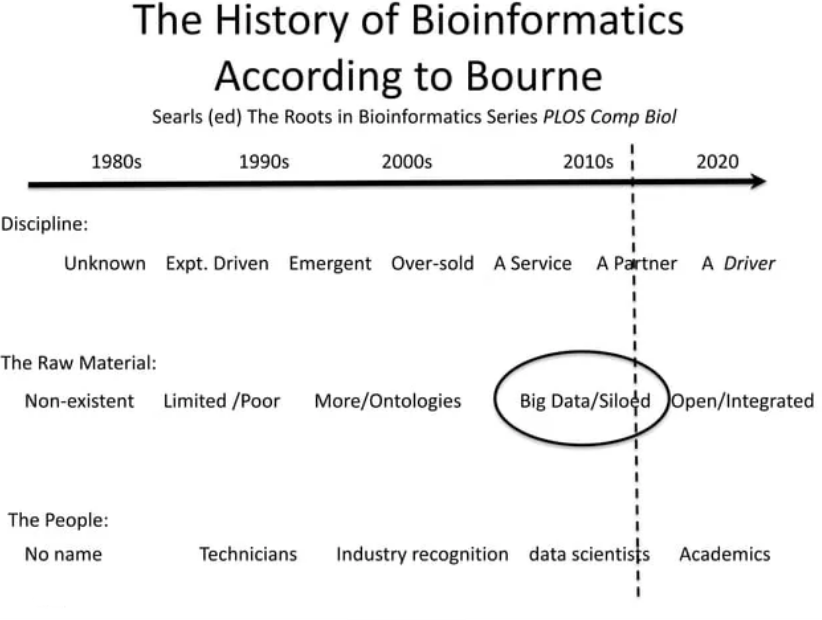
\includegraphics[width = 0.5\textwidth]{figs/history-bioinfo.png}
\caption{Breve historia de la bioinformática en tres niveles: como disciolina, como material que utiliza y como las personas que trabajan en ella. Evolución desde 1980 hasta 2020.}
\end{figure}

\subsection{Avances tecnológicos en secuenciación}
Existen distintos tipos de tecnologías de secuenciación, comúnmente clasificadas en tres generaciones: la primera generación (first generation), la segunda o Next Generation Sequencing (NGS) y la tercera generación. Las dos primeras generaciones se enfocan en la secuenciación de fragmentos cortos de ADN, mientras que la tercera generación permite la lectura de fragmentos largos, facilitando el ensamblaje completo de genomas. Actualmente, uno de los mayores desafíos tecnológicos es detectar variantes de baja frecuencia y realizar secuenciaciones de ADN en células individuales (single-cell sequencing), lo cual tradicionalmente se hacía de forma masiva (“bulk”).

\begin{figure}[htbp]
\centering
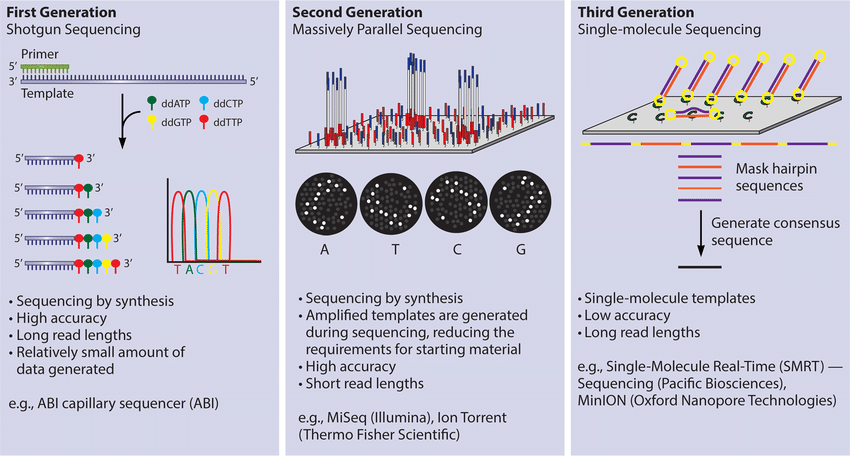
\includegraphics[width = 0.7\textwidth]{figs/sequencing-generations.png}
\caption{Las tres generaciones de secuenciación y su forma de actuar.}
\end{figure}

A medida que el costo de la secuenciación ha disminuido y la capacidad de almacenamiento ha mejorado desde 1990, los datos generados también han crecido exponencialmente. En un experimento de secuenciación, los costos abarcan tanto la secuenciación en sí como el procesamiento bioinformático, el reporte y el almacenamiento de los datos. La comunidad científica y muchos journals requieren que los datos de proyectos financiados públicamente estén disponibles en bases de datos accesibles, lo que asegura la transparencia y el acceso a esta información valiosa. Para obtener una cobertura de calidad, el ADN suele secuenciarse al menos 30 veces, lo que genera archivos de gran tamaño, como los archivos FastQ, que almacenan información de secuencia y calidad para cada base.

\subsection{Procesos de llamada y priorización de variantes}
Los datos de secuenciación se procesan en pipelines bioinformáticas que comienzan con archivos FastQ normalmente comprimidos y pasan por varias etapas: control de calidad, alineamiento y llamada de variantes (variant calling). Las variantes identificadas pueden incluir cambios de nucleótidos, variaciones en el número de copias de segmentos genómicos (copy number variation) o reordenamientos estructurales.

\begin{figure}[htbp]
\centering
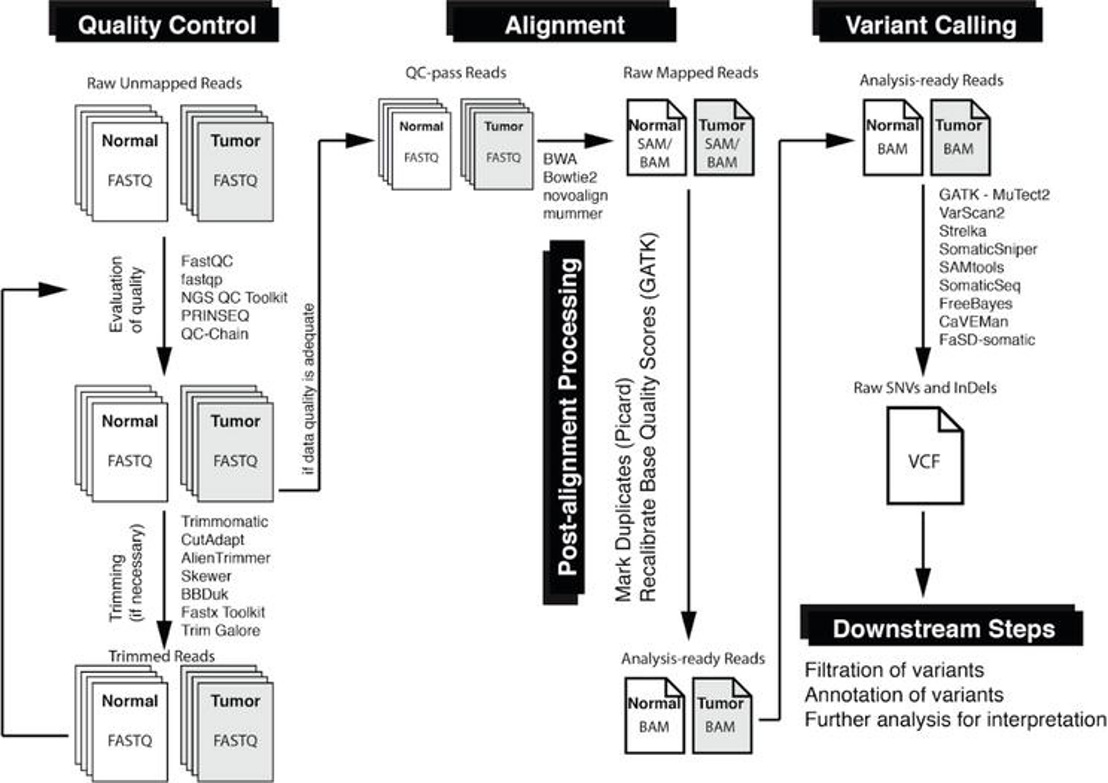
\includegraphics[width = 0.7\textwidth]{figs/bioinfo-pipeline.png}
\caption{Esquema de la pipeline que se sigue en bioinformática para la llamada de variantes.}
\end{figure}

La priorización de variantes se basa en factores como el impacto funcional, la frecuencia alélica en la población y la asociación con enfermedades. Sin embargo, muchas variantes requieren validación experimental, frecuentemente en modelos animales como ratones, para corroborar su relevancia funcional. El proceso de filtrado inicial se enfoca en variantes en exones de genes candidatos, analizando su frecuencia, patogenicidad y modelo de herencia; en caso de no hallarse variantes relevantes, se amplía el análisis a variantes oligogénicas o no codificantes.

\begin{figure}[htbp]
\centering
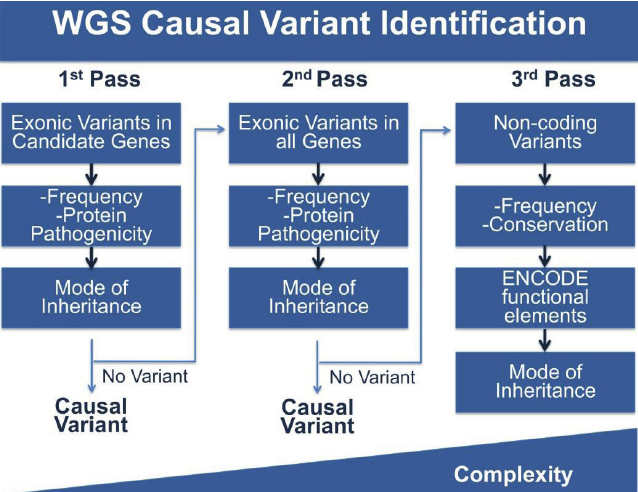
\includegraphics[width = 0.5\textwidth]{figs/variant-priorization.png}
\caption{Ejemplo de la priorización de variantes.}
\end{figure}

\subsection{Genómica en medicina de precisión}
La genómica ha transformado el enfoque de la medicina de precisión, permitiendo identificar enfermedades con bases genéticas, ambientales o una combinación de ambas. Algunas variantes genéticas confieren una predisposición a enfermedades sin ser causantes directas, lo cual es crucial para inferir relaciones causales y acelerar ensayos clínicos mediante la integración de grandes volúmenes de datos. Estas variantes pueden clasificarse en germinales (heredadas) o somáticas (adquiridas).

\begin{figure}[htbp]
\centering
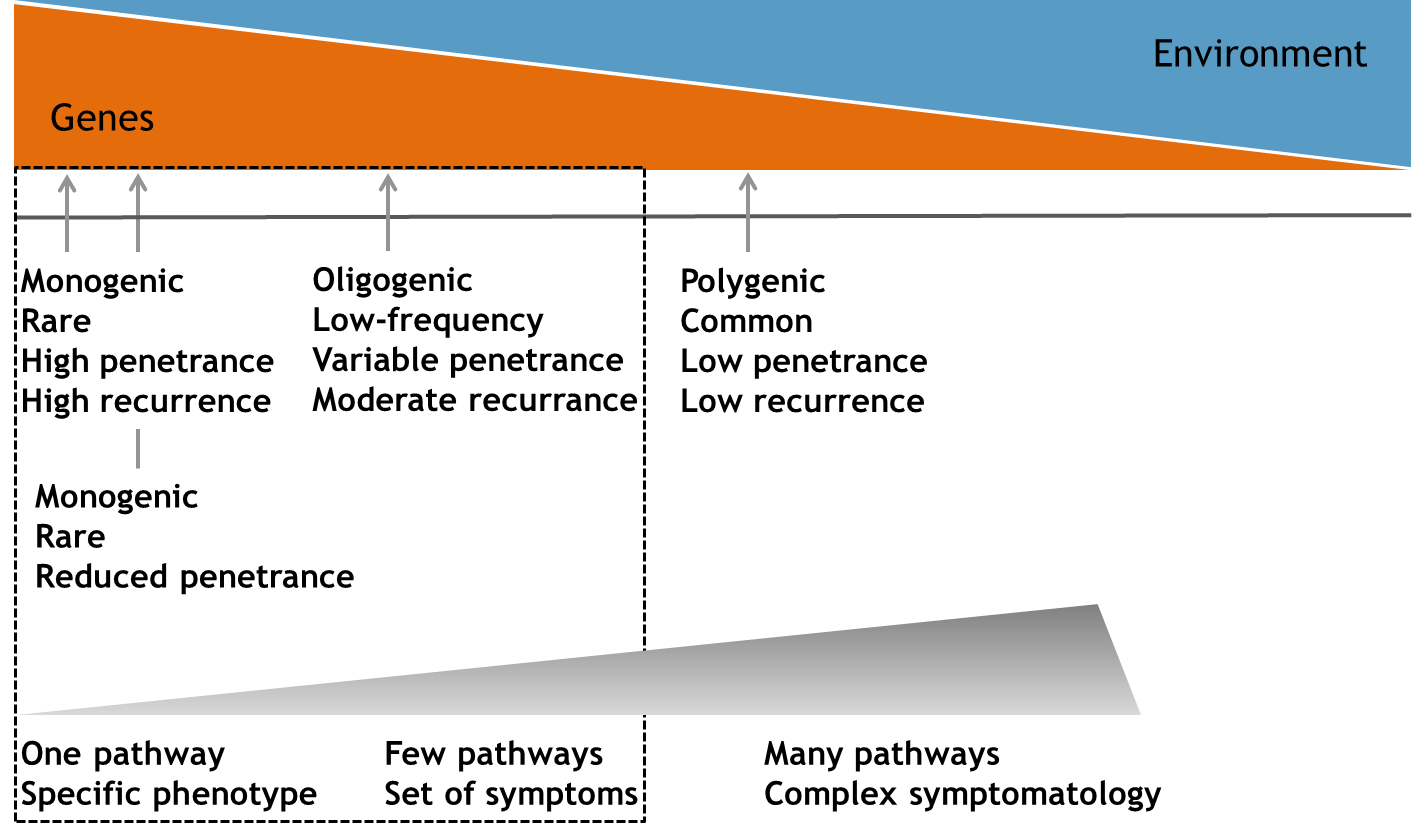
\includegraphics[width = 0.5\textwidth]{figs/genetic-environment.png}
\caption{Representación gráfica de la relación entre enfermedades con base genética, ambientales o una mezcla de ambas.}
\end{figure}

En medicina de precisión, la genómica es solo una capa de datos entre muchas. Para una comprensión holística de la salud y la enfermedad, es necesario combinarla con información de otras “ómicas” como la transcriptómica, epigenómica, proteómica, metabolómica, y datos de microbioma. Además, los datos clínicos y epidemiológicos también forman parte del ecosistema de \textbf{Big Data Biomédico}, que actualmente se maneja mediante técnicas avanzadas de computación en clusters HPC, computación en la nube y algoritmos de GPU.

\begin{figure}[htbp]
\centering
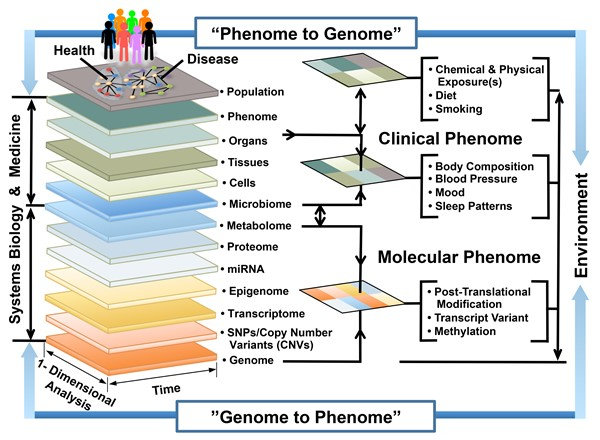
\includegraphics[width = 0.7\textwidth]{figs/bigger-picture-bioinfo.jpg}
\caption{Esquema representando el dibujo general de la bioinformática.}
\end{figure}

Varias bases de datos públicas permiten estudiar la transición entre salud y enfermedad. El estudio de Farmingham, por ejemplo, lleva más de 70 años recolectando datos de factores de riesgo cardiovascular en más de 15,000 participantes. En Reino Unido, el Biobank y, en Estados Unidos, la iniciativa All of Us, también representan recursos de gran envergadura. En España, el CNIC (Centro Nacional de Investigaciones Cardiovasculares) realiza el estudio PESA (Progression of Early Subclinical Atherosclerosis), que ha contribuido a identificar factores predictivos de aterosclerosis subclínica mediante el estudio multiómico, generando nuevos indicadores con un mayor poder predictivo de la formación de placas de colesterol.

\paragraph{Epigenética y la medición de la edad biológica}
El perfil de metilación del ADN es un factor epigenético que puede modificar la expresión genética y se ha utilizado para calcular la “edad biológica” o epigenética de una persona, lo que puede servir como predictor de esperanza de vida y salud. Al comparar estos perfiles con la edad cronológica, sexo y otros factores, se obtiene información sobre el envejecimiento y el riesgo de enfermedades, facilitando el desarrollo de estrategias de salud personalizadas.

\subsection{Resumen}
La genómica ha liderado una revolución científica en el siglo XX, evolucionando desde el estudio de componentes individuales hasta una perspectiva integral de sistemas biológicos y de investigación basada en datos masivos. La bioinformática se ha convertido en una disciplina central en el análisis genómico y predicción de estructuras proteicas, impulsada por el Proyecto Genoma Humano y el desarrollo de tecnologías de secuenciación. Los avances actuales buscan no solo la secuenciación del ADN, sino también la integración de estos datos con datos epidemiológicos y moleculares para obtener una comprensión más profunda de la salud y la enfermedad. Así, el Proyecto Genoma Humano fue decisivo para sentar las bases de tecnologías de secuenciación, el desarrollo de la bioinformática en sí y el uso social e industrial de los datos ómicos.

La identificación de características genómicas relevantes causales de rasgos/enfermedades se basa en la anotación de variantes en bases de datos y en estudios poblacionales: hay margen de mejora y un gran éxito de la ciencia colaborativa. Hoy en día, los principales proyectos tratan no sólo de secuenciar el ADN, sino de integrar esta información con datos epidemiológicos y otros datos moleculares para comprender mejor la salud y la enfermedad.
Las enfermedades, en función de su base genética, pueden clasificarse en monogénicas (mendelianas), oligogénicas (ej., cardiopatías familiares) y complejas (evaluadas mediante puntuaciones de riesgo poligénicas). Esta clasificación permite avanzar en la medicina de precisión, abordando enfermedades desde su origen genético para ofrecer intervenciones de salud más efectivas y personalizadas.

%30/10 - Álvaro
\section{Métodos de secuenciación}
La secuenciación permite pasar de la información contenida en el ADN a un dominio digital mediante una representación abstracta. 

El primer método de secuenciación fue desarrollado por Maxam-Gilbert utilizando un marcador 5'. El ADN se trató con distintos químicos para romperlo de forma diferencial dependiendo de la base. Según la ruptura, se ponía en un gel de acrilamida y se realizaba una electroforesis. El revelado se hacía por autoradiografía de rayos X. En base al patrón de las bandas, se obtenía la secuencia. 

El siguiente método es el método de la terminación de cadena o Sanger. Se utilizaban deoxinucleótidos, que en el grupo 2' de la pentosa tiene H en lugar de OH. Así, el extremo 5', que se une al extremo 3', no se puede unir, parando la reacción en cadena. Se obtienen moléculas de distinto tamaño a las que se va a realizar lo mismo: se añade un isótopo radioactivo unido a los distintos dinucleótidos en distintos pocillos para realizar una electroforesis. Esta técnica se modificó para utilizar fluoróforos en lugar de isótopos radioactivos. En lugar de detectar el patrón de bandas, se podía poner todo en un pocillo y medir los colores y, de ahí, la secuencia. 
¿Cuál es la clave de este método de secuenciación? El elemento clave es el uso de dideoxinucleótidos, que permiten parar la reacción en cadena de la polimerasa. (Esto saldrá en el examen)

Posteriormente se desarrolló el primer secuenciador, que fue ABI370. Podía secuenciar 5000 bases al día, tardando 16.000 años para secuenciar todo el genoma humano. Este secuenciador suponía pasar de utilizar geles a electroforesis capilar, teniendo una solución con un detector de fluorescencia. A finales de los 90 y principios de los 2000 empezó el Proyecto Genoma Humano, queriendo secuenciar todo el genoma de un ser humano. Empezó en una empresa pública, pero pasó a una empresa privada. Empezó como una competición entre ambos, pero finalmente aunaron esfuerzos, ya que sus técnicas se complementaban.

Con este proyecto se desarrolló el secuenciador ABI377 con varios capilares. El genoma tiene zonas altamente repetitivas (telómeros y centrómeros) que son muy difíciles de secuenciar, y hasta el año pasado no salió el paper que lo describía.

Los métodos que se utilizaron en el proyecto fueron los siguientes:

Hierarchical shotgun:
se clonaba y por enzima de restricción se sacaban fragmentos que se secuenciaban. Así, se iba solapando la información de los distintos fragmentos, obteniendo los contigs. Los contigs se iban solapando para obtener la secuencia original.

Whole-genome shotgun:
Es prácticamente igual, pero en lugar de partir de cromosomas bacterianos se hacía directamente del genoma. Se clonaba en bacterias, se cogía el ADN y se realizaba la misma aproximación de solapamiento. 

La electroforesis capilar iba pasando los fragmentos de distinto tamaño por el capilar. Hay un detector que pilla la señal de fluorescencia y genera la lectura de la secuencia de unos 500 pares de bases.

Cuando se empezó a secuenciar, el costo era bastante alto, pero con el tiempo el precio fue bajando (mediante técnicas diferentes a Sanger).

NGS: la siguiente ola de tecnología de secuenciación del ADN
NGS hace referencia a la secuenciación de segunda generación. Se realiza de forma paralela y masiva, lo que se conoce como high-throughput sequencing. Los métodos de secuenciación son 454 Roche, Solexa Illumina, ABI/SOLiD, Complete Genomics, Pacific Biosciences, Ion Torrent y Oxford Nanopore. 

Preparación de librerías de NGS
Una librería de secuenciación consiste enc oger el material genético y generar una serie de secuencias que son las que luego van al secuenciador. El output del secuenciador son las lecturas (reads). La característica de la segunda generación es que utiliza la molécula de ADN original y, sobre ella, la amplifica, es decir, la utiliza como molde para generar muchas moléculas iguales. Así, primero se fragmenta el ADN para generar el molde, se amplifica clonalmente en beads (bolitas con primers que permiten que la secuencia se pegue y se amplifique), en fase sólida (es un cristal en el que se pega la molécula que se amplifica) o nanobolas (la amplificación no ocurre en fase sólida, si no circular, generando un ovillo que se secuencia sobre una placa metálica funcionalizada, es decir, con grupos químicos que permite que se adhiera). Al final se obtiene una bola o una placa con el ADN amplificado que se secuencia todo a la vez. Esto permite secuenciar de forma paralela todas las moléculas, permitiendo así un alto rendimiento o high-throughput. 

Se pueden distinguir dos tipos de métodos de secuenciación de segunda generación: secuenicación por síntesis o por ligamiento.  La distinción viene por la enzima principal. Por síntesis, es la polimerasa, y por ligación la ligasa. 

Secuenciación por síntesis
Se puede distinguir por la terminación de ciclos reversibles o por adición de nucleótidos.

Terminación del ciclo reversible (CRT)
Es la evolución del método Sanger. Se basa en utilizar dNTPs bloqueados en el extremo 3' OH. En Sanger, este grupo no estaba (eran dideoxinucleótidos), bloqueando la duplicación de la polimerasa. En este caso está bloqueado, por lo que a efectos prácticos es lo mismo. Partiendo del template, este template se une a los beads o al cristal. Una vez unido, se añade la mezcla de la reacción, que va a tener la polimerasa y el dNTP con el grupo 3'OH bloqueado y un fluoróforo. El fluoróforo va a decir qué nucleótido sería el siguiente en la secuencia. Al unirse el fluoróforo, se emite una señal. Como en la placa se ha amplificado clonalmente el template, cada copia va a emitir la señal y se recibe la señal del cluster. En el siguiente ciclo, se desbloquea el grupo OH y se permite la unión 5'-3'. Así, se repite el ciclo: se añaden nucleótidos bloqueados, se recibe la señal y se desbloquea con un químico de lavado. El microscopio que detecta la señal fluorescente tiene un límite de detección, por lo que es necesaria la amplificación. Además, la placa con los moldes tiene en los límites unos marcadores que permiten que el microscopio se enfoque a la altura a la que debe. 

Una vez terminada la secuenciación, se utiliza como primer para secuenciar la cadena contraria. Esto se debe a que el microscopio va enfocando peor y se pierde calidad. Cada señal emitida por el fluoróforo se conoce como call o llamada. Cada call tiene una confident score de Q, que se calcula mediante:
$$Q = - 10 log_{10} P $$

Por tanto, si Q es 30, P sería $10^{-3}$, representando P la probabilidad de error. La información que se obtiene en el archivo es la secuencia obtenida con un valor Q asociado codificado en ASCII. 

Hay microscopios de 2 y de 4 canales. Los microscopios de 4 canales tienen mayor calidad al poder distinguir cada uno de los nucleótidos. Los de 2 canales utilizan la combinación de dos fluoróforos. Esto último detecta verde, rojo, ambos o nada, pero esto último es arriesgado, ya que puede que algunos nucleótidos pierdan el fluoróforo y se considere una G. El de 2 canales es más rápido, pero tiene una peor calidad. Actualmente, se suele realizar con microscopios de 2 canales al ser más rápido y barato.

El tipo de secuenciador depende del caso de uso y del dinero que se quiera gastar. 

Las ventajas de la secuenciación CRT es que es la que produce la mayor cantidad de secuencias secuenciadas a la vez (mayor throughput). La desventaja es el límite que puede secuenciar, que es en torno a 150 bases por cada extremo. 

Single Nucleotide Addition (SNA)
En cada ciclo de la adición de nucleótidos simple, se añade solo un tipo de nucleótidos. Estos métodos detectan la adición de los nucleótidos. AL terminar el ciclo se lava y se añade otro tipo de nucleótido, midiendo cuántos se han añadido. EL problema son los homopolímeros, es decir, el mismo nucleótido repetido varias veces. Como el extremo OH no se ha incorporado, se pueden añadir varios nucleótidos seguidos, y se necesita que la señal sea proporcional al número de nucleótidos añadidos para que no haya un problema de fase.

Pyrosecuenciación
Este es el primer método que se desarrolló, y está basado en el uso del grupo pirofosfato. Cuando se produce la síntesis del ADN, se libera un grupo pirofosfato. El pirofosfato tiene un enlace de alta energía que se utiliza con la pirofosfatasa acoplada a la luciferasa. Así, se produce una cantidad de luz en función del número de nucleótidos añadidos. 

En este caso, se utilizan beads con un template amplificado clonalmente. Hay una placa con cuarzo transparente enfocado por el secuenciador. En este caso, no es un microscopio que va por posición, si no tipo fotografía. Lo que se hace es poner cada uno de los nculeótidos en cada ciclo, y con eso se va secuenicando. Este método supuso una gran ventaja con Sanger por ser más rápido y barato, y la calidad de la secuenciación es Q45 (99,997\%). El problema está con las secuencias largas, ya que cuando hay un error, hay un cambio de fase. 

Ion Torrent proton detection
Ion Torrent utiliza la medida del cambio de potencial. Cuando se produce la polimerización del ADN, se liebra un protón que produce un cambio de pH y, por tanto, un cambio de voltaje que es detectado. Este método de secuenicación también utiliza beads. Se une un nucleótido y se ve el cambio de potencial. CUando se uenn dos, hay un cambio proporcional a los dos. El problema es que, cuando se unen muchos, el cambio de potencial no es proporcional (si se unen 50, el cambio no es 50x). Por ello, al final de cada cilo hay que lavar para eviar la señal cruzada. 
La ventaja de este método es que es muy barato y es por lo que se utiliza mucho en los hospitales. 

Secuenciación por ligación
Seucenciación por SOLiD
Se basa en la ligación por sondas con do sbases complementarias a la base que se va a unir. En cada ciclo se añade una sonda de 5 en las que 2 se conocen y 3 permiten que se unan a cualquier sitio. Se utiliza con beads. Se utiliza una ligasa que va a unir la sonda a la molécula de ADN. La sonda tiene un fluoróforo, por lo que se ve el color de la sonda. Cuando se ha producido la unión, se elimina el fluoróforo, y se realiza otro ciclo con otra sonda. Así, se mapean dos nucleótidos con espacios de 3. Una vez hecho esto, se repite, añadiendo un espaciador que hace que la sonda se una al siguiente sitio. Al final, cada base está codificada por la suma de dos sondas, y esto se realiza durante 5 ciclos.

Complete Genomics Nanoballs BGI
La amplificación se realiza mediante el rolling circle. Una vez se ha realizado el ovillo, se hibrida en una placa y se utilizan sondas que por ligación y por el fluoróforo se indica el nucleótido al que se unen. Se va secuenciando de manera iterativa cada uno de los nucleótidos. La ventaja es que permite una alta densidad de bolas, tiene una precisión muy alta. No obstante, permite secuenciar lecturas pequeñas y, al final, se utilizan distintos adaptadores a los que se unen las sondas, permitiendo aumentar el througput. Hay partes de la tecnología que no se conocen y está principalmente disponible en China.

Importante a quedar claro: diferencia entre secuenciación por síntesis y por ligación, y dentro de ellos la diferencia entre el método CRT y SNA. Los métodos de ligación hay que saber que existen, pero no es habitual trabajar con ellos. 

Uno de los problemas que más se intenta tratar en la secuenicación de segunda generación es la tasa de error, que está en torno a un Q25-Q35. Al secuenciar mucha cantidad de bases, hay errores elevados en la secuenciación. Es imporatnte remarcar que aunque ilumina diga que tienen muy poco error porque tienen un Q30 y sus lecturas son de 150 pares de bases, realmente se leen muchas secuencias a la vez.
Además, como las lecturas de segunda generación son pequeñas, es difícil construir genomas completos, y hay problemas a la hora de variantes estructurales. Hay errores de secuenciación en regiones complejas y repetitivas (AT o CG en SBS y homopolímeros en SNA). El coste de los equipos es muy caro. Hay un sesgo en la amplificación a la hora de la construcción de la librería, ya que hay regiones que se amplifican mejor y regiones en las que peor. Cuantos más ciclos, peor calidad. SI en uno de lso pasos no se incorpora un nucleótido, se produce el fenómeno de la cadena retrasada, habiendo un descabalgamiento del ciclo de lectura real y el ciclo de lectura en el que creemos que estamos. Al secuenciar en un cluster, cuando se produce un error en el cluster, el error se queda a lo largo de la secuenciación (si hay un error en el ciclo 1, se mantiene durante todos los demás). Además, hay cambios epigenéticos.

Take-home messages